% Valentino Vranic
% Metody inzinierskej prace 2012/13

\documentclass{beamer}

%\usetheme{Warsaw}
%\usetheme{Antibes}
\usetheme{JuanLesPins}
%\usetheme{Goettingen}

\usecolortheme{seahorse}
%\usecolortheme{dolphin}
%\usecolortheme{rose}
% http://deic.uab.es/~iblanes/beamer_gallery/index_by_color.html
%\usecolortheme{beaver}

%\useoutertheme[]{sidebar}

\setbeamercovered{transparent}

\usepackage[slovak]{babel}
\usepackage[T1]{fontenc}
\usepackage[utf8]{inputenc}
\usepackage{url}
\usepackage{graphicx}
\graphicspath{ {./images/} }
\usepackage{listings}

\lstset{language=C++,basicstyle=\fontsize{8}{9.6}\selectfont,showstringspaces=false,columns=fullflexible,identifierstyle=\ttfamily,keywordstyle=\bfseries,showstringspaces=false,columns=fullflexible}
%\lstset{language=C,basicstyle=\fontsize{10.5}{12.6}\selectfont,identifierstyle=\ttfamily,keywordstyle=\bfseries,showstringspaces=false,columns=fixed}

\def\BibTeX{\textsc{Bib}\kern-.08em\TeX} 

\newcommand{\footcite}[1]{\footnote{\tiny #1}}
\newcommand{\umlet}{.5}
\newcommand{\emp}[1]{\textit{\alert{#1}}}
\newcommand{\kw}[1]{\mbox{\textbf{#1}}}
\newcommand{\id}[1]{\texttt{#1}}
\newcommand{\stl}{\guillemotleft}
\newcommand{\str}{\guillemotright}

\newcommand{\lsti}{\lstinline[basicstyle=\fontsize{10.5}{12.1}\selectfont]}

\newcommand{\ssection}[1]{
	\section{#1}
	\begin{frame}[fragile=singleslide]\frametitle{}
	\Huge #1
	\end{frame}
}

\newcommand{\ssectionn}[1]{
	\section*{#1}
	\begin{frame}[fragile=singleslide]\frametitle{}
	\Huge #1
	\end{frame}
}

\newenvironment{program}{\begin{beamercolorbox}[rounded=true,shadow=true]{block body}\vspace{-4mm}}{\vspace{-2mm}\end{beamercolorbox}}

\setbeamercolor{fvystup}{fg=white,bg=black}
\newenvironment{vystup}{\begin{beamercolorbox}[rounded=true,shadow=true]{fvystup}}{\end{beamercolorbox}}

\newenvironment{poznamka}{\begin{beamercolorbox}[rounded=true,shadow=false]{block body}}{\end{beamercolorbox}}

\setbeamertemplate{footline}[page number]
{
%\insertpagenumber
%\begin{beamercolorbox}{section in head/foot}
%\vskip2pt\insertnavigation{\paperwidth}\vskip2pt
%\end{beamercolorbox}%
}



\author{Lukáš Michalčák}
%\url{www.fiit.stuba.sk/~vranic}, \url{vranic@fiit.stuba.sk}}
%{\tiny \url{www.fiit.stuba.sk/~vranic}, \url{vranic@fiit.stuba.sk}}
\institute{
	%Ústav informatiky, informačných systémov a softvérového inžinierstva\\
	Fakulta informatiky a informačných technológií\\
	Slovenská technická univerzita v Bratislave}

\subtitle{\vspace{3mm} Metódy inžinierskej práce 2019/2020}

\title{Holistický prístup k tvorbe serióznych hier
}

\date{\footnotesize 22. november 2022}




\begin{document}

\begin{frame}[fragile=singleslide]
\titlepage
\end{frame}


\begin{frame}[fragile=singleslide]\frametitle{Úvod}
Úvod do prezentácie, motivujeme čitateľa, uvedieme v skratke problém (viď názov), používame bežne odrážky.


\end{frame}


\begin{frame}[fragile=singleslide]\frametitle{Nedostatky serióznych hier}
%\tableofcontents
V bodoch:

\begin{itemize}
\item Odrážky na prvej úrovni
\item Môže ich byť viac
	\begin{itemize}
	\item Toto je už druhá úroveň
	\item Ďalšia odrážka
	\end{itemize}
\item Pokračuje prvá úroveň
\end{itemize}
\end{frame}


%\section{Nejaká časť}
% príkaz \ssection by vytvoril zvláštný slajd s názvom časti - v krátkych prezentáciách to prekáža, lebo oberá o čas

\begin{frame}[fragile=singleslide]\frametitle{Teórie učenia a koncepcie herného vývoja}
\begin{itemize}
\item Odrážky na prvej úrovni
\item Môže ich byť viac
	\begin{itemize}
	\item Toto je už druhá úroveň
	\item Ďalšia odrážka
	\end{itemize}
\item Pokračuje prvá úroveň
\end{itemize}

\end{frame}



%\section{Ďalšia časť}

\begin{frame}[fragile=singleslide]\frametitle{Predostrenie optimálnej koncepcie a štruktúry vývoja}
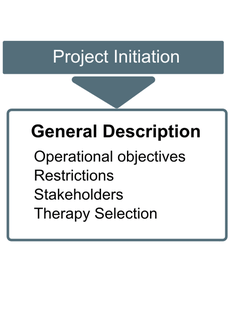
\includegraphics{gameska.png}
\end{frame}


\begin{frame}[fragile=singleslide]\frametitle{Zhrnutie}


\end{frame}





\end{document}
